\documentclass[prb,aps,twocolumn,showpacs,10pt]{revtex4-1}
\pdfoutput=1
\usepackage{dcolumn}% Align table columns on decimal point
\usepackage{bm}% bold math

%\usepackage{anysize}
\usepackage[colorlinks,hyperindex, urlcolor=blue, linkcolor=blue,citecolor=black, linkbordercolor={.7 .8 .8}]{hyperref}
\usepackage{graphicx}
%\usepackage{tabularx}
\usepackage{amsfonts}
\usepackage{amsmath}
\usepackage{amssymb}
\usepackage{amsbsy}
\usepackage{tikz}
%\usepackage{wrapfig}
%\usepackage{setspace}
%\usepackage{caption}
%\usepackage{fancyhdr}
\usepackage{nicefrac}
\usetikzlibrary{arrows,shapes,positioning}
\newenvironment{psmallmatrix}
  {\left[\begin{matrix}}
  {\end{matrix}\right]}


\newcommand{\etal}{{\it et~al.}}

\graphicspath{{benchmark/}}

\begin{document}

\title {Project 2}

\author{Jane Kim}
\affiliation{Physics 480: Computational Physics}
\date{\today}


\begin{abstract}
\noindent Abstract\\
\end{abstract}



\maketitle

\section{Introduction}

Many problems in physics are difficult, if not impossible, to solve analytically. However, in many cases, they can be reduced to relatively simple eigenvalue problems which can be solved numerically. In this project, we developed an eigenvalue and eigenvector solver using Jacobi's algorithm for real, symmetric matrices in order to solve three different examples of such problems with varying levels of complexity.
\subsection{Buckling Beam}
For the simplest of the three problems, we consider a beam of length $L$, whose vertical displacement in the $y$-direction is $u(x)$ for $x \in [0,L]$. If $R$ is some constant which reflects the properties, such as the rigidity, of the beam and a force $F$ is applied at $x=L$ towards the origin, the vertical displacement $u(x)$ satisfies the differential equation
\begin{equation}
R\frac{d^2 u(x)}{dx^2} = -Fu(x),
\end{equation}
with homogenous boundary conditions $u(0)=u(L)=0$. Since different combinations of the physical paramters $F, R$, and $L$ can yield the same solution, it is beneficial to introduce the dimensionless quantity $\rho = \frac{x}{L}$ to scale the differential equation. Then (1) becomes
\begin{equation}
\frac{d^2 u(\rho)}{d\rho^2} = -\lambda u(\rho),
\end{equation}
where $\lambda = FL^2/R$ and $\rho \in [0,1]$. For a given number of mesh points $N$, we can obtain a discretized approximation to $u(\rho)$ by rewriting (2) as an eigenvalue problem given by
\begin{align}
\label{eqn:eqlabel}
\begin{split}
A\vec{u} &= \lambda \vec{u},
\\
\begin{psmallmatrix} d&a& \\
a&d&a\\
&\ddots&\ddots&\ddots\\
&&a&d&a\\
&&&a&d\\
\end{psmallmatrix}
\begin{psmallmatrix}
u_1\\u_2\\ \vdots \\ u_{N-2}\\ u_{N-1}
\end{psmallmatrix}&=
\lambda
\begin{psmallmatrix}
u_1\\u_2\\ \vdots \\ u_{N-2}\\ u_{N-1}
\end{psmallmatrix},\\
u_i &= u(\rho_i),\\
\rho_i &= ih,\\
\end{split}
\end{align}
where $d = 2/h^2$, $a = -1/h^2$, $h = 1/N$ is the step size. At the endpoints, $u_0 = u_N = 0$. This Toeplitz matrix has analytic eigenvalues
\begin{equation}
\lambda_i = d+2a\cos \left( \frac{i \pi}{N+1} \right) , \ \ \ i = 1, 2, ..., N-1,
\end{equation}
which we used to check the accuracy of the eigenvalue solver.

\subsection{One Electron Harmonic Oscillator}
Jacobi's algorithm is applicable for any real, symmetric matrix, so the same program we developed to solve the buckling beam problem can be used to solve the time-independent Schr{\"o}dinger equation for one and two electrons in a three-dimensional harmonic oscillator potential. For one electron with $l=0$, we substitute $R(r)=u(r)/r$ into the radial equation and introduce a dimensionless variable $\rho = r/\alpha$ to obtain
\begin{equation}
\left( -\frac{\hbar^2}{2m\alpha^2} \frac{d^2}{d\rho^2} + \frac{1}{2}m\omega^2\alpha^2\rho^2 \right) u(\rho) = E u(\rho). 
\end{equation}
By fixing $\alpha=(\hbar/m\omega)^{1/2}$ and letting $\lambda=2m\alpha^2 E/\hbar^2 = 2E/\hbar\omega$, (5) becomes 
\begin{equation}
\left( -\frac{d^2}{d\rho^2} + \rho^2 \right) u(\rho) = \lambda u(\rho).
\end{equation}
The boundary conditions are $u(0)=\lim_{\rho \rightarrow \infty} u(\rho)=0$, but due to the finite nature of discretizing the differential equation, we must define a window $[\rho_{min}, \rho_{max}]$ on which to compute the eigenvalues and eigenvectors. Then the discretized equation is given by
\begin{equation}
-\frac{1}{h^2} u_{i-1} + \left( \frac{2}{h^2} + \rho_i^2 \right) u_i -\frac{1}{h^2} u_{i+1} = \lambda u_i, 
\end{equation}
where $h=(\rho_{max}-\rho_{min})/N$, $\rho_i = \rho_{min} + ih$, $i = 1, ..., N-1$. Therefore, the only difference between this eigenvalue problem and the buckling beam problem is that the diagonal elements have an additional non-constant term $\rho_i^2$. This problem also has analytic eigenvalues given by $\lambda = 3, 7, 11, 15, ...$ .

EIGENVALUE CALCULATIONS ARE MOST ACCURATE WHEN WINDOW CONTAINS VALUES OF RHO FOR WHICH THE CORRESPONDING EIGENVECTOR (OR U(RHO)) IS NOT IDENTICALLY $\approx 0$

\subsection{Two Electron Harmonic Oscillator}

When the repulsive Coulomb interaction is ignored, the Hamiltonian $H_0$ for two electrons in a harmonic oscillator can be written with respect to the center-of-mass coordinate $\mathbf{R}=(\mathbf{r}_1+\mathbf{r}_2)/2$ and the relative coordinate $\mathbf{r}=\mathbf{r}_1-\mathbf{r}_2$:
\begin{align}
\label{eqn:eqlabel}
\begin{split}
H_0(r,R) &= H_0(r) + H_0(R)\\
H_0(r) &=-\frac{\hbar^2}{m} \frac{d^2}{dr^2} + \frac{1}{4} k r^2\\
H_0(R) &= -\frac{\hbar^2}{4m} \frac{d^2}{dR^2} + kR^2
\end{split}
\end{align}
where $k=m\omega^2$. Then with the Coulomb interaction
\begin{equation}
V(r) = \frac{\beta e^2}{r}, \ \ \ \beta e^2 = 1.44 \ \text{eV} \cdot \text{nm}
\end{equation}
the $r$-dependent Schr{\"o}dinger equation is given by
\begin{equation}
H(r)\psi(r)=[H_0(r)+V(r)]\psi(r)=E_r \psi(r)
\end{equation}
As with one electron case, we substitute the dimensionless variable $\rho=r/\alpha$ in (10) to obtain
\begin{equation}
\left( -\frac{d^2}{d\rho^2} + \omega_r^2\rho^2 + \frac{1}{\rho}\right) \psi(\rho) = \lambda\psi(\rho).
\end{equation}
Here, we have defined $\alpha=\hbar^2/m\beta e^2$ and $\lambda = $ 
$m\alpha^2E/\hbar^2$. Thus the two electron case simply adds another term $\rho_i$ to the diagonal elements of $A$ from the one electron case. 

\section{METHOD}


The two-fluid model provides a means of explaining some of the strange properties of HeII. This model considers HeII to have two separate components: the normal fluid component and the superfluid component. The former behaves like a typical fluid, while the latter is said to have zero entropy and zero viscosity. Above the lambda point, liquid helium consists entirely of the normal fluid component. But as it is cooled below $T_\lambda$, the superfluid component increases until the liquid helium is completely superfluid at absolute zero.  


The corresponding densities of the two components, $\rho_n$ and $\rho_s$, sum to the total density of the liquid $\rho$ and the mass flux $\mathbf{j}$ of the superfluid is given by:
\begin{equation}
\mathbf{j}=\rho_n \mathbf{v}_n+\rho_s \mathbf{v}_s,
\end{equation}
where $\mathbf{v}_n$ and $\mathbf{v}_s$ are the velocities of the normal and superfluid components, respectively \cite{stanford}. It can be shown that mass, momentum, and entropy conservation produce two different wave equations. The solution to the first equation
\begin{equation}
\frac{\partial^2\rho}{\partial t^2} = u_1^2 \nabla^2 \rho,
\end{equation}
is a pressure (or density) wave with speed of sound $u_1$. In first sound, the velocities of each component are equal, so the elastic energy of deformation travels as a single wave. Thus the relative densities of the two components remain constant.\\

The solution to the second equation
\begin{equation}
\frac{\partial^2S}{\partial t^2} = u_2^2 \nabla^2 S,
\end{equation}
is a heat (or entropy) wave with speed of second sound $u_2$. In second sound, we have that $\mathbf{j}=\rho_n \mathbf{v}_n+\rho_s \mathbf{v}_s=0$, so the relative densities of the two components oscillate, while the total density remains constant\cite{stanford}. As $T\rightarrow 0$, $\rho_s$ approaches $\rho$ and $\rho_n$ approaches 0. \\

It should be noted, however, that helium-4  is a boson so the two "components" of the fluid are merely theoretical aids. In other words, this model is inaccurate, but it provides a meaningful framework of understanding the phenomenon of second sound. \\

\section{Experiment}

\subsection{Apparatus}
The speeds of first and second sound were measured by detecting the various resonance frequencies of a transducer cavity. Identical sets of Nucleopore filters and capacitive transducers were placed on either end of the cylindrical brass cavity, which had length $L=4.0$ cm and radius $r = 0.5$ cm (FIG. 1).\\

\begin{figure}
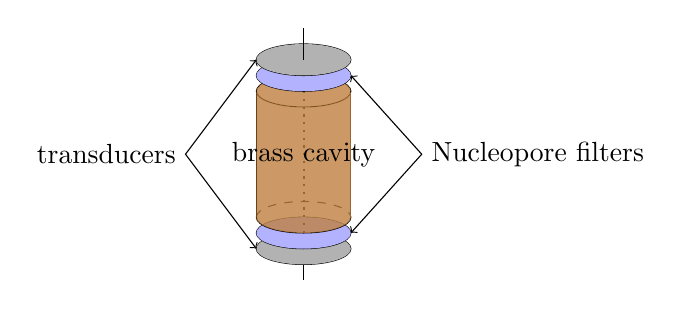
\begin{tikzpicture}

\draw (0,-1.8) -- (0,-2.4);
\draw (0,-2) ellipse (0.6 and 0.2);
\fill [black!30] (0,-2) ellipse (0.6 and 0.2);
\draw (0,-1.8) ellipse (0.6 and 0.2);
\fill [blue!30] (0,-1.8) ellipse (0.6 and 0.2);

\draw (0,0) ellipse (0.6 and 0.2);
\draw [dotted,thick](0,0) -- (0,-1.8);
\fill [brown,opacity=0.8] (0,0) ellipse (0.6 and 0.2);
\draw (-0.6,0) -- (-0.6,-1.6);
\draw (-0.6,-1.6) arc (180:360:0.6 and 0.2);
\draw [dashed] (-0.6,-1.6) arc (180:360:0.6 and -0.2);
\draw (0.6,-1.6) -- (0.6,0);  
\fill [brown,opacity=0.8] (-0.6,0) -- (-0.6,-1.6) arc (180:360:0.6 and 0.2) -- (0.6,0) arc (0:180:0.6 and -0.2);

\draw (0,0.2) ellipse (0.6 and 0.2);
\fill [blue!30] (0,0.2) ellipse (0.6 and 0.2);
\draw (0,0.4) ellipse (0.6 and 0.2);
\fill [black!30] (0,0.4) ellipse (0.6 and 0.2);

\draw (0,0.8) -- (0,0.4);

\node[anchor=center] at (0,-0.8) {brass cavity};
\draw[<->] (-0.6,0.4) -- (-1.5,-0.8) -- (-0.6,-2);
\node[anchor=east] at (-1.5,-0.8) {transducers};
\draw[<->] (0.6,0.2) -- (1.5,-0.8) -- (0.6,-1.8);
\node[anchor=west] at (1.5,-0.8) {Nucleopore filters};

\end{tikzpicture}
\caption{The transducer cavity setup. One transducer produces sound waves by applying an oscillating electric field, which causes the Nucleopore filters to apply a force on the liquid in the cavity. The transducer on the other end detects the sound waves. }
\end{figure}

The Nucleopore filters are thin polymer membranes with metallized and grounded surfaces. One transducer applies an electric field that oscillates the membranes, producing a sound wave. The pores of the filters are so small that the normal fluid component is blocked. But as mentioned before, the superfluid component has zero viscosity, so it can freely flow through the membranes with no loss in kinetic energy. This replicates the conditions for second sound, since the relative densities of the two components are allowed to oscillate while maintaining constant total density. These sound waves are detected by the transducer on the other end of the cavity.\\

For a standing wave resonance to occur, the length of the cavity must be a half-integer multiple of the wavelength of the driving oscillations\cite{phy}:
\begin{equation}
L=\frac{n \lambda}{2}, \ \ \ \ n \in \mathbb{Z}.
\end{equation}

\noindent By the dispersion relation $u = \lambda f$, we have that the frequency difference between adjacent resonances is given by
\begin{equation}
\Delta f = \frac{u}{\lambda_{n+1}} - \frac{u}{\lambda_n} = \frac{u}{2L}( n+1-n )= \frac{u}{2L}.
\end{equation}
Thus, we can calculate the speed of first or second sound using
\begin{equation}
u = 2L\Delta f.
\end{equation}

The transducer chamber was placed inside two glass dewars (FIG. 2). To avoid rupturing the thin Nucleopore filters with an extreme drop to liquid helium temperatures ($\sim$ 4 K), the apparatus was first cooled to liquid nitrogen temperatures ($\sim$ 77 K). This was accomplished by filling the experimental chamber with 1 atm of N$_2$ gas and the liquid nitrogen chamber with liquid nitrogen. The outer vacuum chamber was remained sealed, and the inner vacuum chamber was allowed to have a small amount of N$_2$ gas to help facilitate the cooling process. 

\subsection{Electronics}

A full diagram of the experiment is shown in FIG. 2. A waveform generator was used to send a driving signal with some frequency $f$ to the top transducer of the resonant cavity. The sound waves were then detected by the bottom transducer and sent to an SR830 lock-in amplifier. Lock-in amplifiers take accurate measurements of small AC signals that have the same frequency and phase as a reference signal. In this experiment, the reference signal was the driving signal from the waveform generator.\\

The lock-in amplifier decomposes a signal $S(t)$ into a sum of the form
\begin{equation}
S(t) = \sum_k A_k \cos(\omega_k t + \phi_k),
\end{equation}
where $A_k$ is the amplitude, $\omega_k$ is the frequency, and $\phi_k$ is the phase of the $k$th wave. Then, it multiplies $S(t)$ by the reference signal $R(t)=A_R\cos(\omega_R t)$ such that
\begin{align*}
R(t)S(t)&=\sum_k A_R A_k \cos(\omega_R t) \cos(\omega_k t)\\
&=\frac{1}{2} A_R \sum_k A_k [\cos((\omega_R-\omega_k)t+\phi_k]\\
& \ \ \ + \cos((\omega_R+\omega_k)t+\phi_k).
\end{align*}
The second term in the summation has a high frequency when $\omega_k \approx \omega_R$, so it can be filtered out by a low pass filter. The lock-in amplifier thereby "picks out" signals which have the same frequency and phase as the reference signal. \\

Now, consider the electric field $E$ between the rigid end of the cavity and the metallized surface of the Nucleopore filters. We can model this interaction with a parallel plate capacitor, where the force exerted on the liquid can be shown to be quadratic in $E$\cite{phy}. Since the electric field oscillates with some frequency $\omega_R$, the force on the filter (and hence the reading on bottom transducer) will appear to have a frequency $2\omega_R$. Since the lock-in amplifier would filter this signal out, a large DC bias voltage was applied to the transistors. (By symmetry, both bias voltages were chosen to be 45 V.) Then, we have
\begin{equation}
F\propto (E_{DC}+E_{AC})^2 = E_{DC}^2 + 2E_{DC}E_{AC} + E_{AC}^2.
\end{equation}
The first term is a constant, the second is linear in $E_{AC}$, and the last is small. Thus, the lock-in amplifier effectively measures signals with the desired frequency. \\

A Cernox resistor, attached to the transducer cavity, was used to monitor the temperature in the experiment chamber. It is only sensitive to temperatures below 40 K, so it was only in use when the experiment chamber was filled with liquid helium. The resistance was measured by a multimeter, and the temperature of the liquid helium was reduced by lowering the vapor pressure above the liquid with a roughing pump. 

\subsection{Procedure}

The apparatus was cooled to liquid nitrogen temperatures for over six hours. At this point, there was 1 atm of N$_2$ gas in the experiment chamber. FIG. 3. shows a full sweep of resonances in the N$_2$ gas during the pre-cooling process. The nitrogen gas was evacuated from the experiment chamber and replaced with 1 atm of helium gas immediately before transferring the liquid helium. In principle, the experiment chamber could have been filled with helium gas at the beginning of the cooling process. But helium can diffuse through glass and conduct heat through the vacuum layers, so we chose to wait on transferring the helium gas until after the pre-cooling procedure.\\


Then, the experiment chamber was filled with liquid helium (LHe) by placing the ends of the transfer line into the storage container and the experiment chamber. Pressurizing the storage container with additional helium gas at $\sim 5$ psi allowed the liquid helium to flow into the chamber. Liquid helium has a very low index of refraction, so the liquid level was not easy to dicern. So other signs were used to monitor the liquid level. The start of the flow was signified by the violent boiling of LHe.  The initial boiling will settle momentarily, until the liquid level approaches the top of the experiment chamber. Then the violent boiling returns due to LHe coming in contact with the warmer region of the apparatus. So, the \textit{second} rapid boiling signifies the experiment chamber is full. \\

Once the liquid helium began to flow into the chamber, the apparatus dropped to $\sim$4 K almost immediately. A sweep of 500-5000 Hz in LHe at 4.15 K is shown on the top panel of FIG. 4. Since second sound is not exhibited by liquid helium at temperatures above the lambda point, we expected no resonance peaks. However, small resonance peaks were recorded for frequencies below ~2kHz, about 120 Hz apart. These peaks were attributed to noise from AC electrical signals that operate at 60 Hz. We suspect that odd harmonics of these signals are amplified in the cavity, resulting in frequency differences of 120 Hz. \\


Controlling the temperature of the fluid was a matter of balancing the effect of the vacuum pump (to lower the temperature) and adding additional helium gas into the chamber (to raise the temperature). The temperature was lowered to 1.78 K and the driving frequencies were swept from 500 to 5000 Hz. The results are shown in the bottom panel of FIG. 4. The second sound peaks were most prominent for frequencies above 3 kHz, so we swept over frequencies 3 kHz to 4 kHz with a step size of 1 Hz.


\section{Results}

Data was collected for five different temperatures below the lambda point and the speed of second sound was calculated using equation (6). The resonance peaks were found manually by searching for local maxima in the lock-in amplitude data. The average frequency difference $\Delta f$ between adjacent resonance peaks and the speed of second sound $u_2$ for each temperature is shown in the table below. The results are shown in FIG. 5. alongside published data from R.J. Donnelly \cite{donnelly.} 

\begin{center}
\begin{tabular}{|c|c|c|c|c|c|}
\hline
$T$ (K) & $\delta T$ (K) & $\Delta f$ (Hz) & $\delta(\Delta f)$ (K) & $u_2$ (m/s) & $\delta u_2$ (m/s)\\
\hline
\hline
1.6727&0.0013&251.3&1.414&20.11&11.06\\
\hline
1.9602&0.0026&232.5&1.414&18.60&10.23\\
\hline
2.0889&0.0034&185.0&1.414&14.80&8.141\\
\hline
2.1451&0.0130&110.7&1.414&8.856&4.872\\
\hline
2.1624&0.0064&65.50&1.414&5.240&2.884\\
\hline
\end{tabular}
\end{center}

The horizontal error bars ($\delta T$) correspond to the variation in temperature during each sweep. The vertical error bars ($\delta u_2$) were calculated with the following:

\begin{equation}
u_2 = 2 L \Delta f = 2 L (f_n-f_{n-1})
\end{equation}
\begin{equation}
\frac{\delta u_2}{u_2} = \sqrt{\left( \frac{\delta L }{L} \right)^2 + \left( \frac{\delta (f_n-f_{n-1}) }{\Delta f} \right)^2}\\ \\
\end{equation}


The error in resonance frequency measurements was determined to be the frequency step size of 1 Hz. So, $\delta (f_n-f_{n-1}) = \sqrt{2}$ Hz. $\delta L$ was estimated as the expected change in the length $L$ due to thermal contraction. The thermal expansion coefficient for brass \cite{toolbox} is $\alpha \approx 18.5 \cdot 10^{-6} K^{-1}$ , so
\begin{equation}
\begin{aligned}
\delta L &\approx \Delta L \\
&= \alpha L \Delta T \\
&\approx(18.5 \cdot 10^{-6}\  K^{-1})(4.0 \ \text{cm})(300 \ K - 2.17 \ K) \\
&= 0.022 \  \text{cm}
\end{aligned}
\end{equation}

All five data points were consistent with the published data \cite{blah}.


\section{Conclusion}
The speed of second sound was measured in HeII for five different temperatures below $T_\lambda$. They agreed with the published data from R.J. Donnelly within the margins of error. We are certain that the peaks we identified were second sound peaks because they appeared only after cooling the liquid nitrogen below the lambda point (FIG. 4). \\


Jacobi algorithm is a brute force way to get eigenvalues, but not very efficient.





\section{Acknowledgements}
I would like to thank my lab partner, Antonius Torode, for taking an entire day to correct our crappy data with me. Special thanks to Jaideep Singh and Johannes Pollanen for providing guidance and insight into the sources of error in our initial attempt of this experiment. 



\newpage
\begin{references}
\bibitem{blah} R.J. Donnelly. "Experimental Superfluidity". University of Chicago Press. 1967. 
\bibitem{toolbox} "Coefficients of Linear Thermal Expansion". The Engineering ToolBox. EngineeringToolBox.com. 
\bibitem{stanford} Otis Chodosh, Jeremy Hiatt, Samir Shah, and Ning Yan. "Second Sound in HeII". Department of Physics, Stanford University. March 21, 2008.
\bibitem{phy} "Second Sound in Superfluid Liquid He". Department of Physics and Astronomy, Michigan State University. PHY 451.
\bibitem{nwe} "Superfluidity". New World Encyclopedia. October 28, 2015. 
\end{references}

\end{document}
